\PassOptionsToPackage{table}{xcolor}

\documentclass[
%	handout,
	notes=none,
	aspectratio=169
]{beamer}

% Comment out the following line to hide the notes
%\setbeameroption{show notes}

% Imports
\usepackage{listings}
\usepackage{amsfonts}
\usepackage{amsmath}
\usepackage{pythonhighlight}
\usepackage{pgfpages}
\usepackage{tabularx}
\usepackage{ifxetex,ifluatex}
\usepackage{etoolbox}
\usepackage{framed}

\mode<handout>{%
	\pgfpagesuselayout{8 on 1}[a4paper,border shrink=5mm]
	\setbeameroption{show notes}
}

% Graphics configuration
\graphicspath{{./graphics/}}
\DeclareGraphicsExtensions{.pdf,.jpeg,.png,.jpg,.pdf}
\definecolor{rctabbg}{rgb}{0.965,0.965,0.965}

% Useful macros
\def\etal{{\it et al.}}
\def\etc{{\it etc.}}
\def\eg{{\it e.g.}}
\def\ie{{\it i.e.}}
\def\cf{{\it cf.}}
\def\qv{{\it q.v.}}
\def\qqv{{\it qq.v.}}
\def\st{s.t.\ }
\def\code{\tt}
\def\setsep{:}
\def\concat{\mathbin{|}}

\renewcommand{\thefootnote}{\fnsymbol{footnote}}
\newcommand{\prescite}[1]{\footnote{\cite{#1}}}
\newcommand{\prestext}[1]{\footnotetext{\cite{#1}}}
\newcommand{\emaillink}[1]{\href{mailto:#1}{\nolinkurl{#1}}}

\setlength{\parskip}{0.5em}

% Tables

\newcolumntype{L}[1]{>{\raggedright\arraybackslash\tiny}p{#1}}

% Program listings
\definecolor{listingbaground}{rgb}{.9,.9,.9}

\lstset{
	language=C,
	backgroundcolor=\color{listingbaground},
	extendedchars=true,
	basicstyle=\fontsize{5pt}{6pt}\ttfamily,
	showstringspaces=false,
	showspaces=false,
	numbers=left,
	numberstyle=\fontsize{5pt}{6pt}\ttfamily\color{gray},
	numbersep=5pt,
	tabsize=2,
	breaklines=true,
	showtabs=false,
	captionpos=b,
	xleftmargin=5mm,
	escapeinside={££}{££},
	framexleftmargin=5mm
}

% https://tex.stackexchange.com/questions/89574/language-option-supported-in-listings
\lstdefinelanguage{JavaScript}{
	keywords={typeof, new, true, false, catch, function, return, null, catch, switch, var, if, in, while, do, else, case, break},
	keywordstyle=\color{blue}\bfseries,
	ndkeywords={class, export, boolean, throw, implements, import, this},
	ndkeywordstyle=\color{darkgray}\bfseries,
	identifierstyle=\color{black},
	sensitive=false,
	comment=[l]{//},
	morecomment=[s]{/*}{*/},
	commentstyle=\color{purple}\ttfamily,
	stringstyle=\color{red}\ttfamily,
	morestring=[b]',
	morestring=[b]"
}

\lstdefinelanguage{QML}{
	keywords={typeof, new, true, false, catch, function, return, null, catch, switch, var, if, in, while, do, else, case, break, id, property, bool, string, int, decimal, target},
	keywordstyle=\color{blue}\bfseries,
	ndkeywords={Page, Example, Timer, Column, PageHeader, TextSwitch, Label},
	ndkeywordstyle=\color{teal}\bfseries,
	identifierstyle=\color{black},
	sensitive=true,
	comment=[l]{//},
	morecomment=[s]{/*}{*/},
	commentstyle=\color{green}\ttfamily,
	stringstyle=\color{red}\ttfamily,
	morestring=[b]',
	morestring=[b]"
}

\lstdefinelanguage{cpp}{
	keywords={class, public, private, try, throw, catch, this, return, null, switch, if, while, do, else, case, break, for, bool, void, const},
	keywordstyle=\color{blue}\bfseries,
	ndkeywords={Q_OBJECT, Q_CLASSINFO, Q_PROPERTY, Q_SLOTS, Q_SIGNALS, signals, slots, READ, WRITE, NOTIFY},
	ndkeywordstyle=\color{teal}\bfseries,
	identifierstyle=\color{black},
	sensitive=false,
	comment=[l]{//},
	morecomment=[s]{/*}{*/},
	commentstyle=\color{purple}\ttfamily,
	stringstyle=\color{red}\ttfamily,
	morestring=[b]',
	morestring=[b]"
}

\lstdefinelanguage{sh2}{
	keywords={dbus, send, zypper, python3},
	keywordstyle=\color{blue}\bfseries,
	ndkeywords={session, type, print, reply, dest},
	ndkeywordstyle=\color{teal}\bfseries,
	identifierstyle=\color{black},
	sensitive=false,
	comment=[l]{\#},
	morecomment=[s]{/*}{*/},
	commentstyle=\color{purple}\ttfamily,
	stringstyle=\color{red}\ttfamily,
	morestring=[b]',
	morestring=[b]"
}

\lstdefinelanguage{shell}{
	basicstyle=\small\ttfamily,
	keywords={python, python3, pip, pip3, srun, sbatch},
	keywordstyle=\color{cyan},
	ndkeywords={torch, distributed, launch},
	ndkeywordstyle=\color{teal}\bfseries,
	identifierstyle=\color{white},
	sensitive=false,
	comment=[l]{\#},
	morecomment=[s]{/*}{*/},
	commentstyle=\color{green}\ttfamily,
	stringstyle=\color{green}\ttfamily,
	morestring=[b]',
	morestring=[b]"
}

% To allow the theme files to be placed in a subdirectory
\makeatletter
	\def\beamer@calltheme#1#2#3{%
		\def\beamer@themelist{#2}
		\@for\beamer@themename:=\beamer@themelist\do
		{\usepackage[{#1}]{\beamer@themelocation/#3\beamer@themename}}}

	\def\usefolder#1{
		\def\beamer@themelocation{#1}
	}
	\def\beamer@themelocation{}

% Quotation styling
% conditional for xetex or luatex
\newif\ifxetexorluatex
\ifxetex
  \xetexorluatextrue
\else
  \ifluatex
    \xetexorluatextrue
  \else
    \xetexorluatexfalse
  \fi
\fi
%
\ifxetexorluatex%
  \usepackage{fontspec}
  \newfontfamily\quotefont[Ligatures=TeX]{\rmdefault} % selects Libertine as the quote font
\else
  \usepackage[utf8]{inputenc}
  \usepackage[T1]{fontenc}
  \newcommand*\quotefont{\fontfamily{\rmdefault}} % selects Libertine as the quote font
\fi

\newcommand*\quotesize{60} % if quote size changes, need a way to make shifts relative
% Make commands for the quotes
\newcommand*{\openquote}
   {\tikz[remember picture,overlay,xshift=-3ex,yshift=-2.5ex]
   \node (OQ) {\quotefont\fontsize{\quotesize}{\quotesize}\selectfont``};\kern0pt}

\newcommand*{\closequote}[1]
  {\tikz[remember picture,overlay,xshift=3ex,yshift={#1}]
   \node (CQ) {\quotefont\fontsize{\quotesize}{\quotesize}\selectfont''};}

% select a colour for the shading
%\definecolor{shadecolor}{HTML}{ffffff}
\definecolor{shadecolor}{rgb}{0.23,0.23,0.23}

\newcommand*\shadedauthorformat{\emph} % define format for the author argument

% Now a command to allow left, right and centre alignment of the author
\newcommand*\authoralign[1]{%
  \if#1l
    \def\authorfill{}\def\quotefill{\hfill}
  \else
    \if#1r
      \def\authorfill{\hfill}\def\quotefill{}
    \else
      \if#1c
        \gdef\authorfill{\hfill}\def\quotefill{\hfill}
      \else\typeout{Invalid option}
      \fi
    \fi
  \fi}
% wrap everything in its own environment which takes one argument (author) and one optional argument
% specifying the alignment [l, r or c]
%
\newenvironment{shadequote}[2][l]%
{\authoralign{#1}
\ifblank{#2}
   {\def\shadequoteauthor{}\def\yshift{-2ex}\def\quotefill{\hfill}}
   {\def\shadequoteauthor{\par\authorfill\shadedauthorformat{#2}}\def\yshift{2ex}}
\begin{snugshade}\begin{quote}\openquote}
{\shadequoteauthor\quotefill\closequote{\yshift}\end{quote}\end{snugshade}}




\usefolder{theme}
\usetheme{TuringDark}

\begin{document}

\title{MPI Part II: Practical MPI}
\subtitle{Converting GPT2 to use MPI and Lightning}
\author{Baskerville Training 2025\\29-30 January 2025 -- David Llewellyn-Jones}
%\date{30 January 2025}

%%%%%%%%%%%%%%%%%%%%%%%%%%%%%%%%%%%%%%%%%

\renewcommand{\thefootnote}{\arabic{footnote}}

\frame{
\titlepage
}
\note{
}

\renewcommand{\thefootnote}{\fnsymbol{footnote}}

%%%%%%%%%%%%%%%%%%%%%%%%%%%%%%%%%%%%%%%%%

\begin{frame}
\frametitle{Message Passing Interface}

\begin{columns}[T]
\begin{column}[T]{1.0\textwidth}
\setlength{\parskip}{0.5em}

\vspace{-0.5cm}
\begin{enumerate}
\setlength{\parskip}{0.5em}
\item MPI: Message Passing Interface
\item Provides a standard for {\it distributed memory parallelisation}
\item Gavin already explained the theory and practice
\item Now let's apply it to some machine learning
\end{enumerate}

\end{column}
\end{columns}

\end{frame}
\note{
}

%%%%%%%%%%%%%%%%%%%%%%%%%%%%%%%%%%%%%%%%

\begin{frame}
\frametitle{Motivation}

\begin{columns}[T]
\begin{column}[T]{1.0\textwidth}
\setlength{\parskip}{0.5em}

\vspace{-0.5cm}
GPUs are great for accelerated training and inference, but processing is bound by:
\begin{enumerate}
\setlength{\parskip}{0.5em}
\item Available memory
\item Speed of computation
\end{enumerate}
How to make AI better?
\begin{enumerate}
\item Improved algorithms
\item Larger models
\item More training data
\end{enumerate}
The last two require {\it more compute}

\end{column}
\end{columns}

\end{frame}
\note{
}

%%%%%%%%%%%%%%%%%%%%%%%%%%%%%%%%%%%%%%%%%

\begin{frame}
\frametitle{Scaling up}

\begin{columns}[T]
\begin{column}[T]{1.0\textwidth}
\setlength{\parskip}{0.5em}

\vspace{-0.5cm}
\begin{enumerate}
\setlength{\parskip}{0.5em}
\item Strong motivation for scaling across GPUs
\item Single device: 4 or 8 GPUs maximum
\item Eventually want to scale across nodes
\item Get this right... the sky's the limit
\end{enumerate}

\end{column}
\end{columns}

\end{frame}
\note{
}

%%%%%%%%%%%%%%%%%%%%%%%%%%%%%%%%%%%%%%%%%

\begin{frame}
\frametitle{Preparation}

\begin{columns}[T]
\begin{column}[T]{1.0\textwidth}
\setlength{\parskip}{0.5em}

\vspace{0.0cm}
\begin{enumerate}
\setlength{\parskip}{0.5em}
\item Open \url{https://docs.baskerville.ac.uk/}
\item Select \href{https://portal.baskerville.ac.uk/}{Baserville Portal}
\item Login if necessary
\item Select \href{https://portal.baskerville.ac.uk/pun/sys/dashboard/batch_connect/sys/bc_bask_jupyter/session_contexts/new}{JupyterLab} from the Interactive Apps list
\item Configure a 2 hour session with 1 GPU on the project {\tt vjgo8416-training25} and the {\tt turing} queue
\item Launch
\end{enumerate}

\end{column}
\end{columns}

\end{frame}
\note{
}

%%%%%%%%%%%%%%%%%%%%%%%%%%%%%%%%%%%%%%%%%

\begin{frame}
\frametitle{}

\begin{columns}[T]
\begin{column}[T]{1.0\textwidth}
\setlength{\parskip}{0.5em}

\vspace{0.0cm}
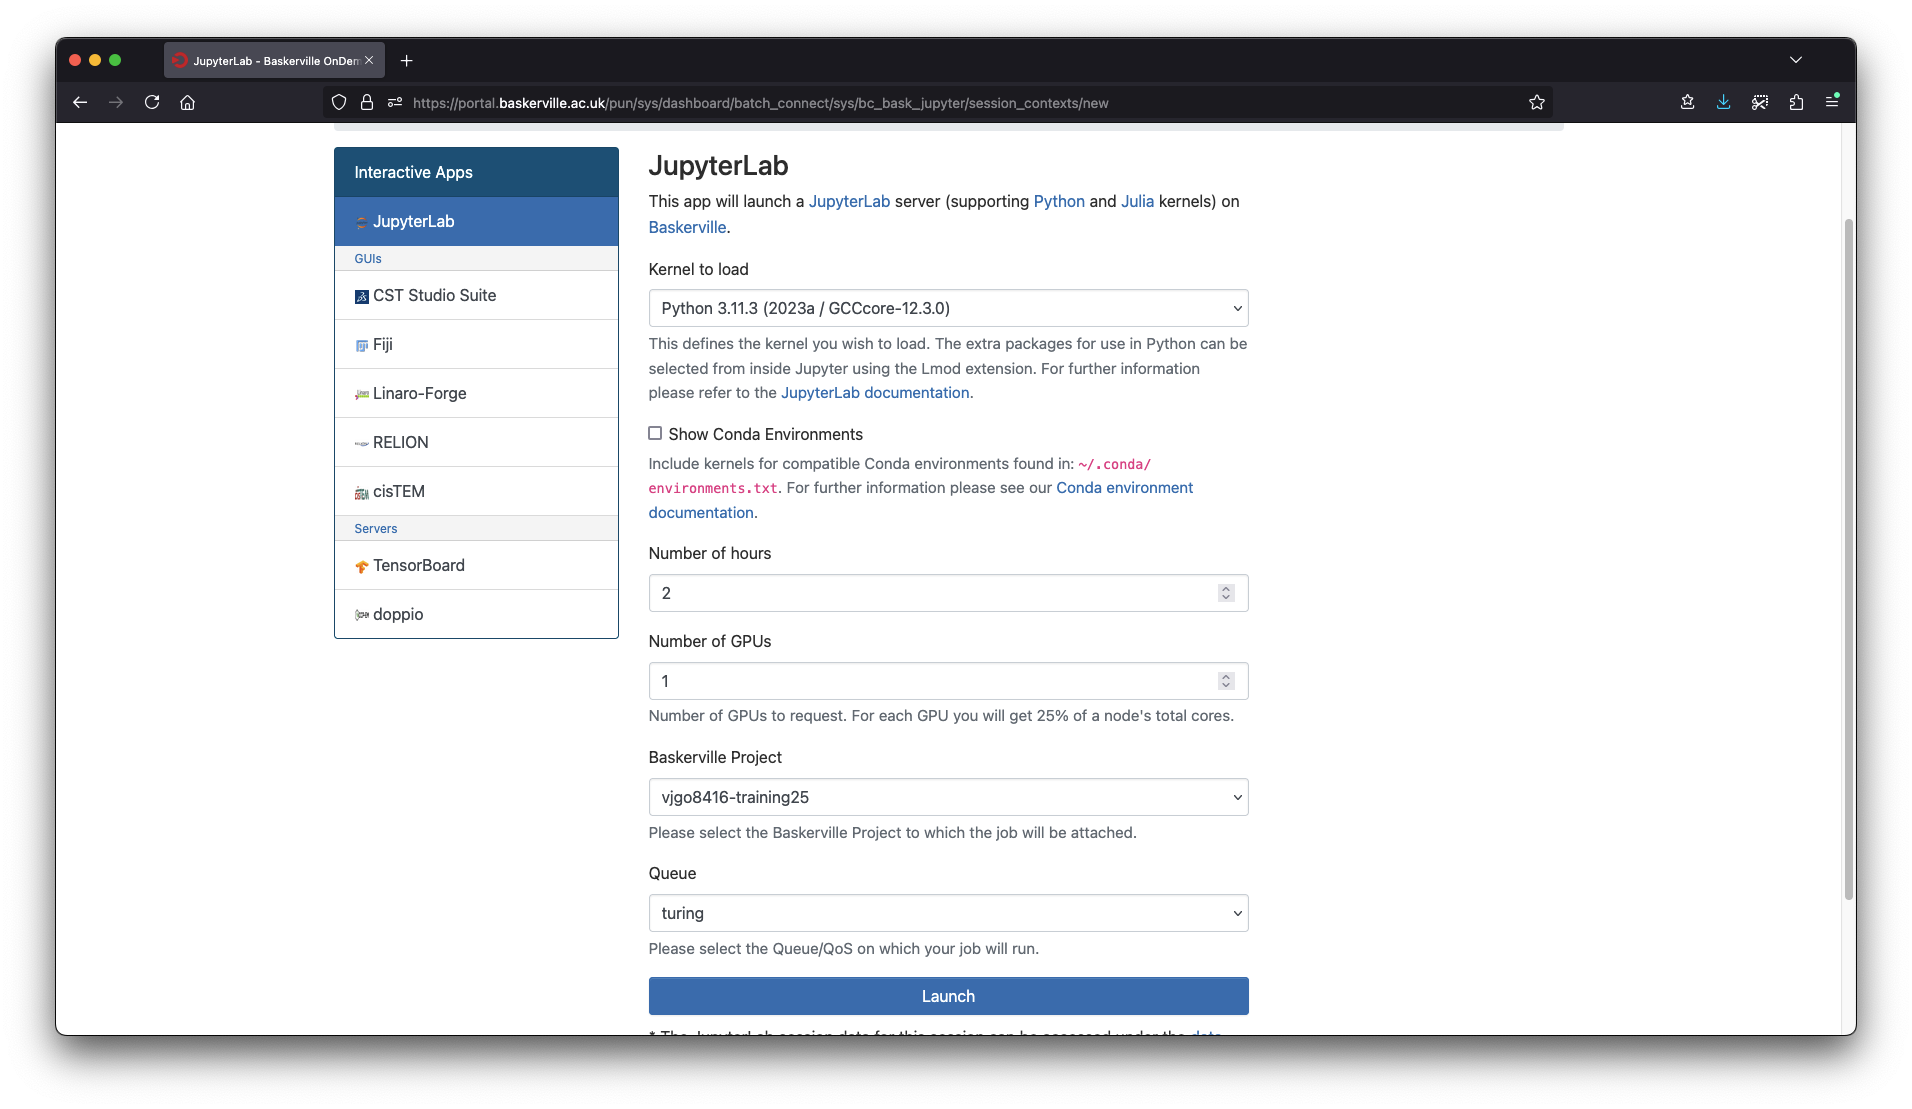
\includegraphics[width=1.0\textwidth]{launch-jupyterlab}


\end{column}
\end{columns}

\end{frame}
\note{
}

%%%%%%%%%%%%%%%%%%%%%%%%%%%%%%%%%%%%%%%%%

\begin{frame}
\frametitle{Types of model parallelism}

\begin{columns}[T]
\begin{column}[T]{1.0\textwidth}
\setlength{\parskip}{0.5em}

\vspace{-0.5cm}
\begin{enumerate}
\setlength{\parskip}{0.5em}
\item DDP: Distributed Data Parallel
\item FSDP: Fully Sharded Data Parallel
\item DeepSpeed ZeRO: Zero Redundancy Optimiser
\end{enumerate}

\end{column}
\end{columns}

\end{frame}
\note{
}

%%%%%%%%%%%%%%%%%%%%%%%%%%%%%%%%%%%%%%%%%

\begin{frame}
\frametitle{Data parallel}

\begin{columns}[T]
\begin{column}[T]{0.9\textwidth}
\setlength{\parskip}{0.5em}

\vspace{-0.5cm}
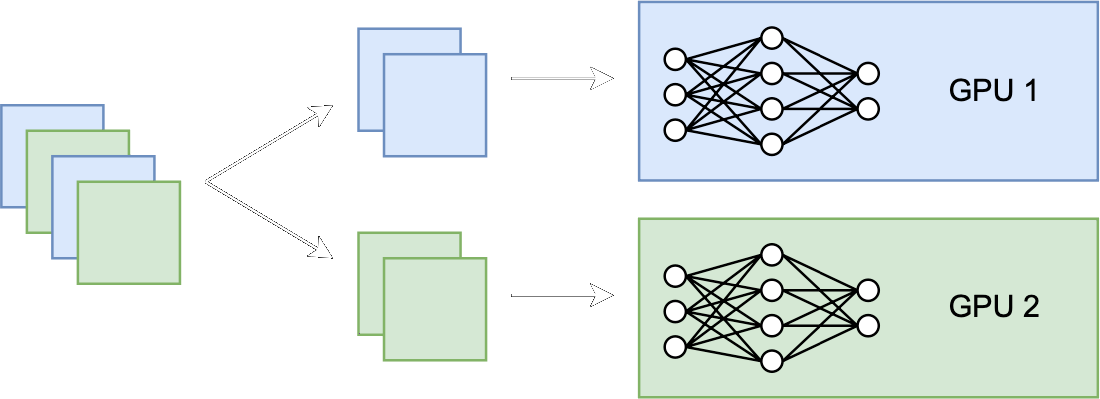
\includegraphics[width=1.0\textwidth]{parallel-data}


\end{column}
\end{columns}

\end{frame}
\note{
}

%%%%%%%%%%%%%%%%%%%%%%%%%%%%%%%%%%%%%%%%%

\begin{frame}
\frametitle{Model parallel FSDP}

\begin{columns}[T]
\begin{column}[T]{0.7\textwidth}
\setlength{\parskip}{0.5em}

\vspace{-1.5cm}
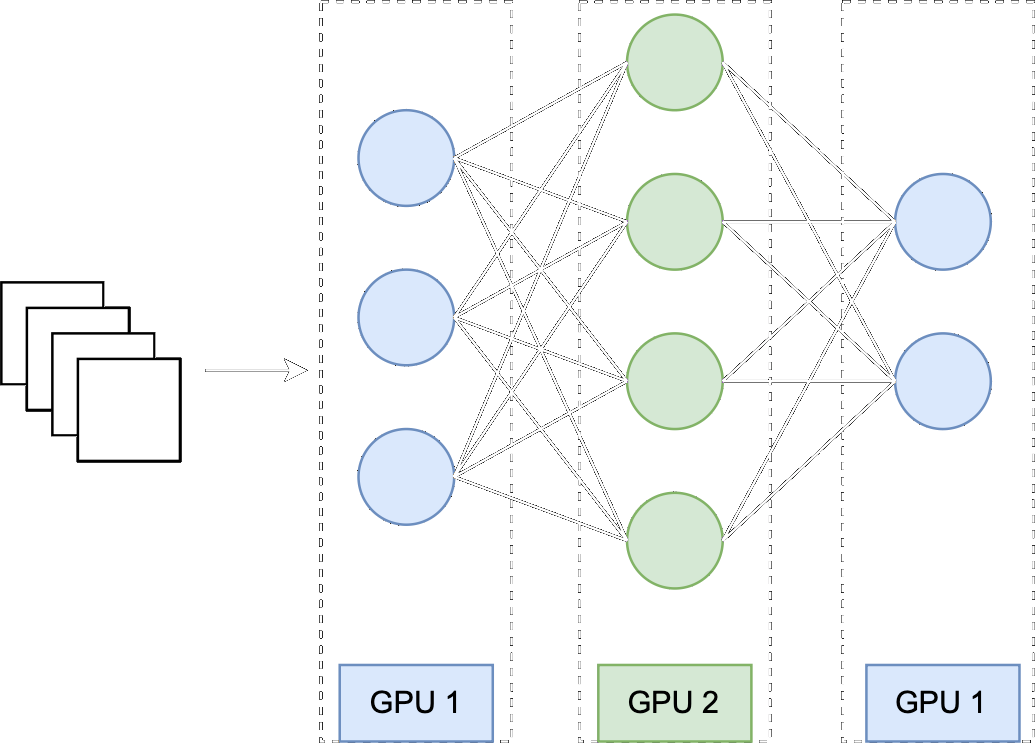
\includegraphics[width=1.0\textwidth]{parallel-vertical}


\end{column}
\end{columns}

\end{frame}
\note{
}

%%%%%%%%%%%%%%%%%%%%%%%%%%%%%%%%%%%%%%%%%

\begin{frame}
\frametitle{Model parallel DeepSpeed}

\begin{columns}[T]
\begin{column}[T]{0.8\textwidth}
\setlength{\parskip}{0.5em}

\vspace{0.0cm}
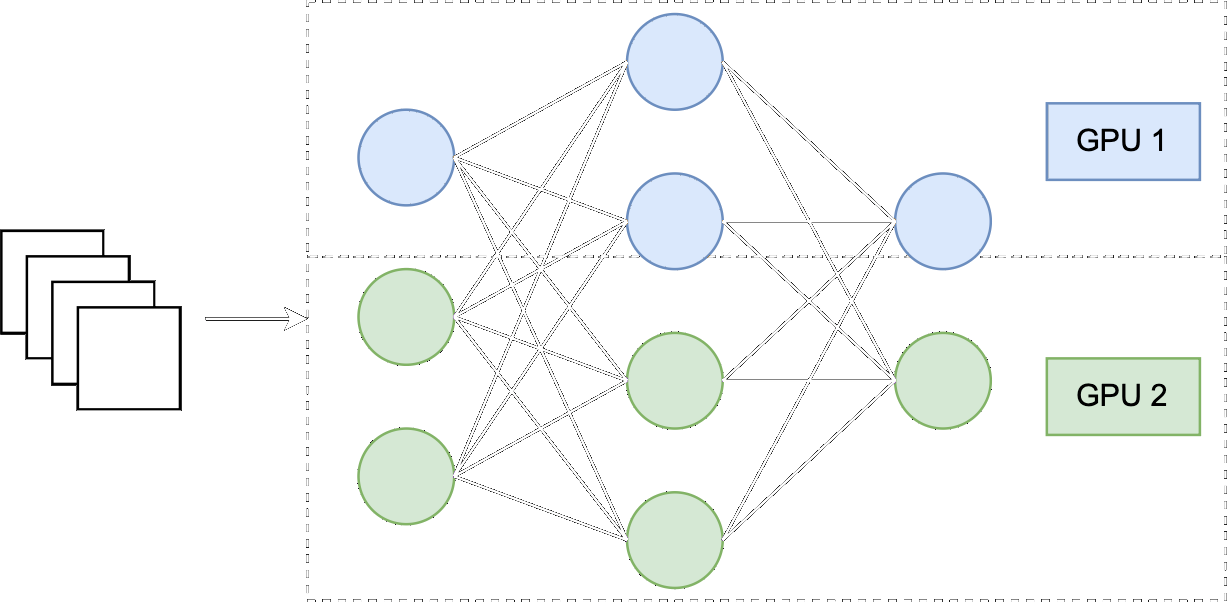
\includegraphics[width=1.0\textwidth]{parallel-horizontal}


\end{column}
\end{columns}

\end{frame}
\note{
}

%%%%%%%%%%%%%%%%%%%%%%%%%%%%%%%%%%%%%%%%%

\begin{frame}
\frametitle{DeepSpeed}

\begin{columns}[T]
\begin{column}[T]{1.0\textwidth}
\setlength{\parskip}{0.5em}

\vspace{-0.5cm}
\begin{enumerate}
\setlength{\parskip}{0.5em}
\item DeepSpeed Stage 1: optimiser state partitioning
\item DeepSpeed Stage 2: gradient partitioning
\item DeepSpeed Stage 3: model parameter partitioning
\end{enumerate}

\end{column}
\end{columns}

\end{frame}
\note{
}

%%%%%%%%%%%%%%%%%%%%%%%%%%%%%%%%%%%%%%%%%

\begin{frame}
\frametitle{The plan}

\begin{columns}[T]
\begin{column}[T]{0.7\textwidth}
\setlength{\parskip}{0.5em}

\vspace{0.0cm}
\begin{enumerate}
\setlength{\parskip}{0.5em}
\item No more theory
\item Simplified GPT2 nano code for one GPU
\item Andrej Karpathy: \url{https://youtu.be/l8pRSuU81PU}
\item Extend to support Distributed Data Parallel
\item Extend using PyTorch Lightning
\end{enumerate}

\end{column}
\begin{column}[T]{0.3\textwidth}
\setlength{\parskip}{0.5em}

\vspace{0.0cm}
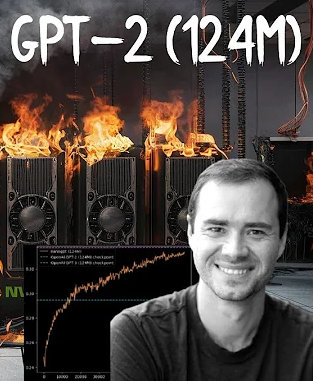
\includegraphics[width=0.9\textwidth]{karpathy}

\end{column}
\end{columns}

\end{frame}
\note{
}

%%%%%%%%%%%%%%%%%%%%%%%%%%%%%%%%%%%%%%%%%

\begin{frame}
\frametitle{The intention}

\begin{columns}[T]
\begin{column}[T]{1.0\textwidth}
\setlength{\parskip}{0.5em}

\vspace{0.0cm}
\begin{enumerate}
\setlength{\parskip}{0.5em}
\item Not to care too much about the model implementation
\item Understand changes needed to add MPI functionality
\item For this, we'll rely heavily on {\tt diff}s
\item Using JupyterLab and SLURM
\end{enumerate}

\end{column}
\end{columns}

\end{frame}
\note{
}

%%%%%%%%%%%%%%%%%%%%%%%%%%%%%%%%%%%%%%%%%

\begin{frame}
\frametitle{Your most important tools}

\begin{columns}[T]
\begin{column}[T]{0.7\textwidth}
\setlength{\parskip}{0.5em}

\vspace{0.0cm}
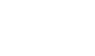
\includegraphics[width=1.0\textwidth]{tools}


\end{column}
\end{columns}

\end{frame}
\note{
}

%%%%%%%%%%%%%%%%%%%%%%%%%%%%%%%%%%%%%%%%%

\begin{frame}
\frametitle{Terminology}

\begin{columns}[T]
\begin{column}[T]{1.0\textwidth}
\setlength{\parskip}{0.5em}

\vspace{0.0cm}
\begin{enumerate}
\setlength{\parskip}{0.0em}
\item Vocabulary: 50257 embeddings
\item Dataset: 9799991296 FineWeb tokens, our training data
\item Sample: a sequence of 1024 tokens from the dataset
\item Microbatch: 32 samples
\item Minibatch (also called a batch): 16 microbatches, gradient accumulation performed afterwards
\item Step: the process for training on one minibatch
\item Epoch: one training sweep of the entire dataset, 18692 steps
\end{enumerate}
\vspace{0.3cm}
$
\qquad \qquad 18692 \times 16 \times 32 \times 1024 = 9799991296
$

\end{column}
\end{columns}

\end{frame}
\note{
}

%%%%%%%%%%%%%%%%%%%%%%%%%%%%%%%%%%%%%%%%%

\begin{frame}
\frametitle{Distributed training}

\begin{columns}[T]
\begin{column}[T]{1.0\textwidth}
\setlength{\parskip}{0.5em}

\vspace{0.0cm}
\begin{enumerate}
\setlength{\parskip}{0.5em}
\item Training on $n$ nodes, each with $m$ GPUs
\item Total $n \times m$ GPUs
\item World size: $w = m \times n$
\item Global rank $r_G$ is a unique index $r_G \in \{ 0, \ldots, w - 1 \}$
\item Local rank $r_L$ is unique per device $r_L \in \{ 0, \ldots, m - 1 \}$
\item No node index, but we do have {\it hostnames}, \eg\/ {\tt bask-pg0309u05a}, {\tt bask-pg0309u06a}
\item We may also have multiple CPU {\it workers\/} for each node
\end{enumerate}

\end{column}
\end{columns}

\end{frame}
\note{
}

%%%%%%%%%%%%%%%%%%%%%%%%%%%%%%%%%%%%%%%%%

\begin{frame}
\frametitle{Training with 1 GPU}

\begin{columns}[T]
\begin{column}[T]{1.0\textwidth}
\setlength{\parskip}{0.5em}

\vspace{0.0cm}
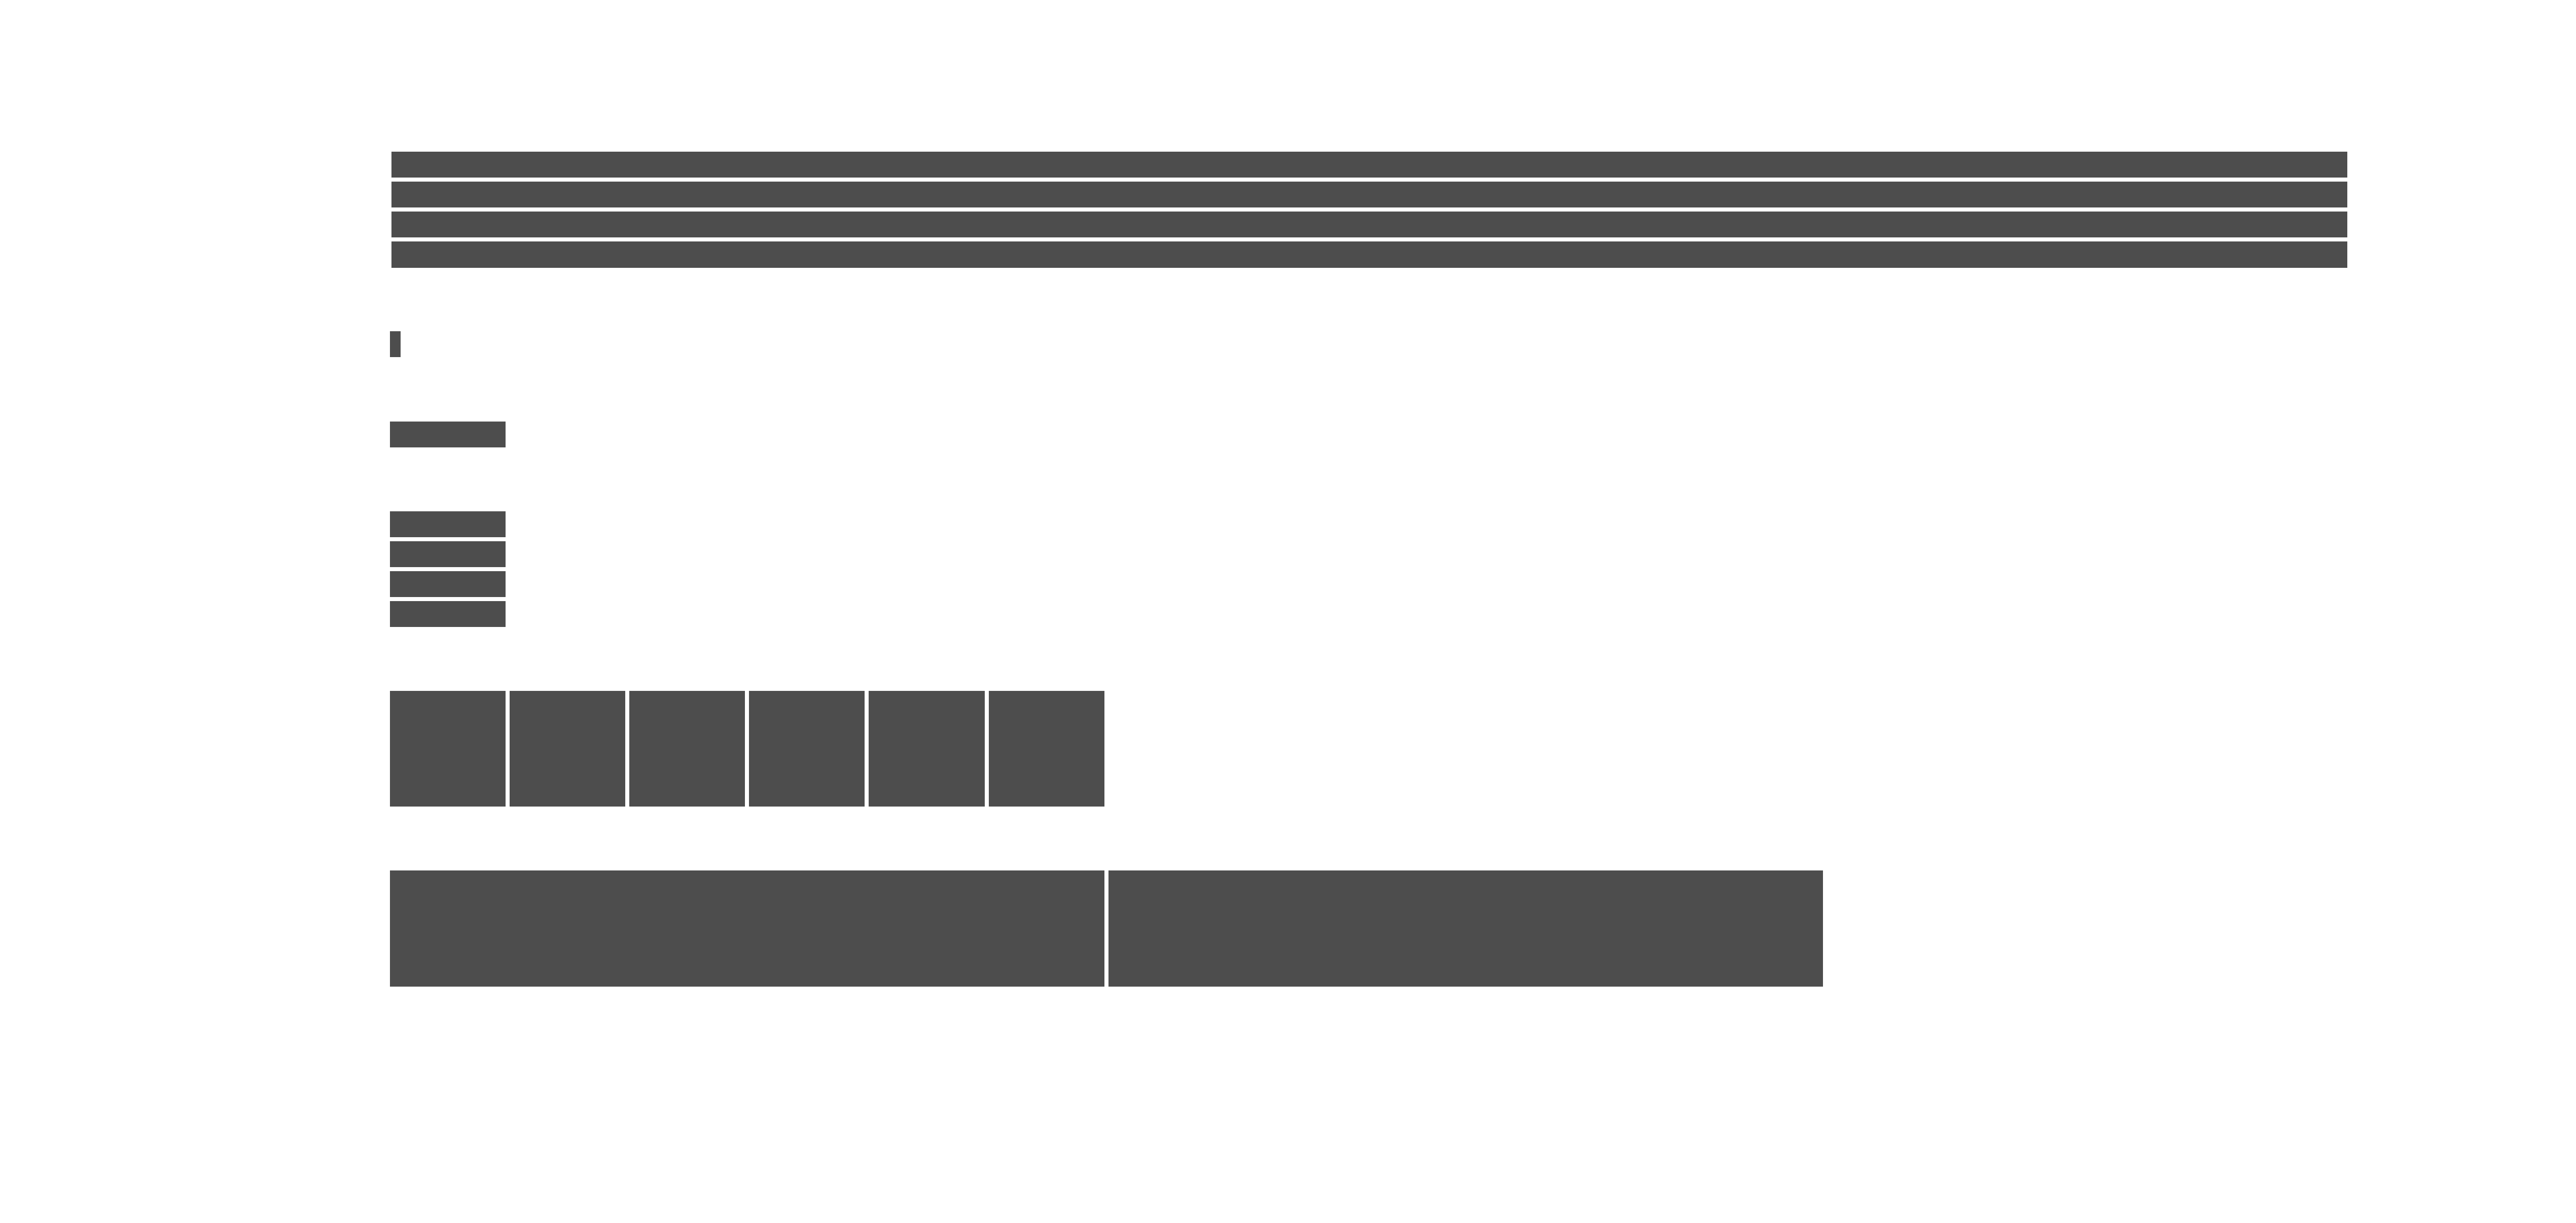
\includegraphics[width=1.0\textwidth]{cadence-1gpu}


\end{column}
\end{columns}

\end{frame}
\note{
}

%%%%%%%%%%%%%%%%%%%%%%%%%%%%%%%%%%%%%%%%%

\begin{frame}
\frametitle{Training with 2 GPUs}

\begin{columns}[T]
\begin{column}[T]{1.0\textwidth}
\setlength{\parskip}{0.5em}

\vspace{0.0cm}
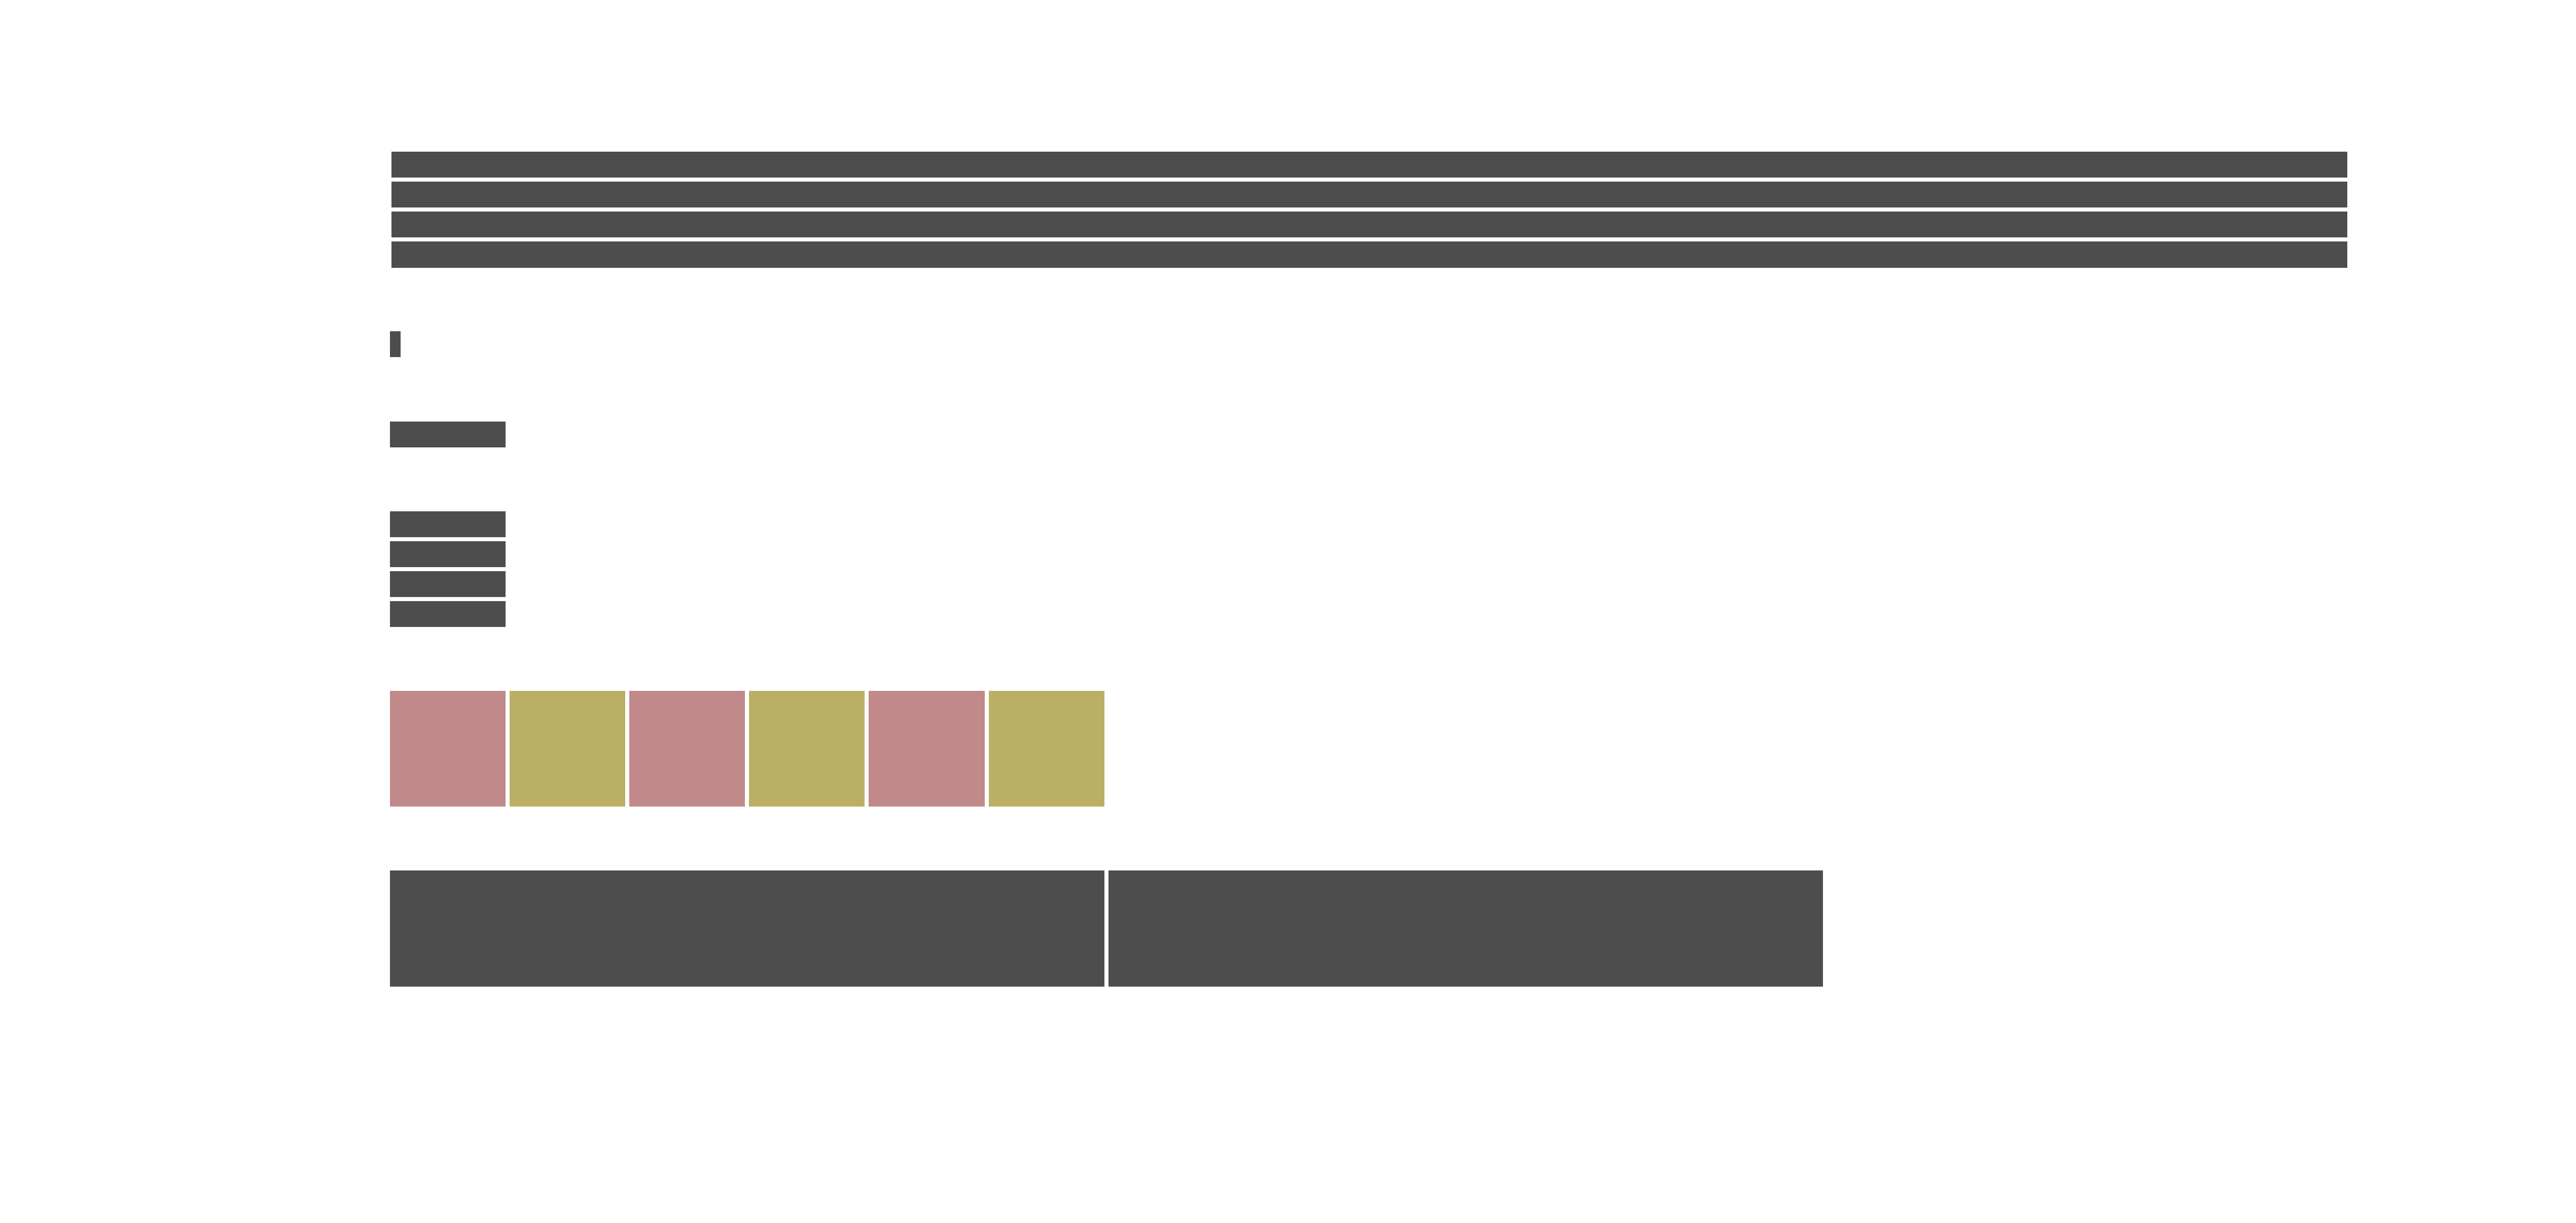
\includegraphics[width=1.0\textwidth]{cadence-2gpu}


\end{column}
\end{columns}

\end{frame}
\note{
}

%%%%%%%%%%%%%%%%%%%%%%%%%%%%%%%%%%%%%%%%%

\begin{frame}
\frametitle{Training with 4 GPUs}

\begin{columns}[T]
\begin{column}[T]{1.0\textwidth}
\setlength{\parskip}{0.5em}

\vspace{0.0cm}
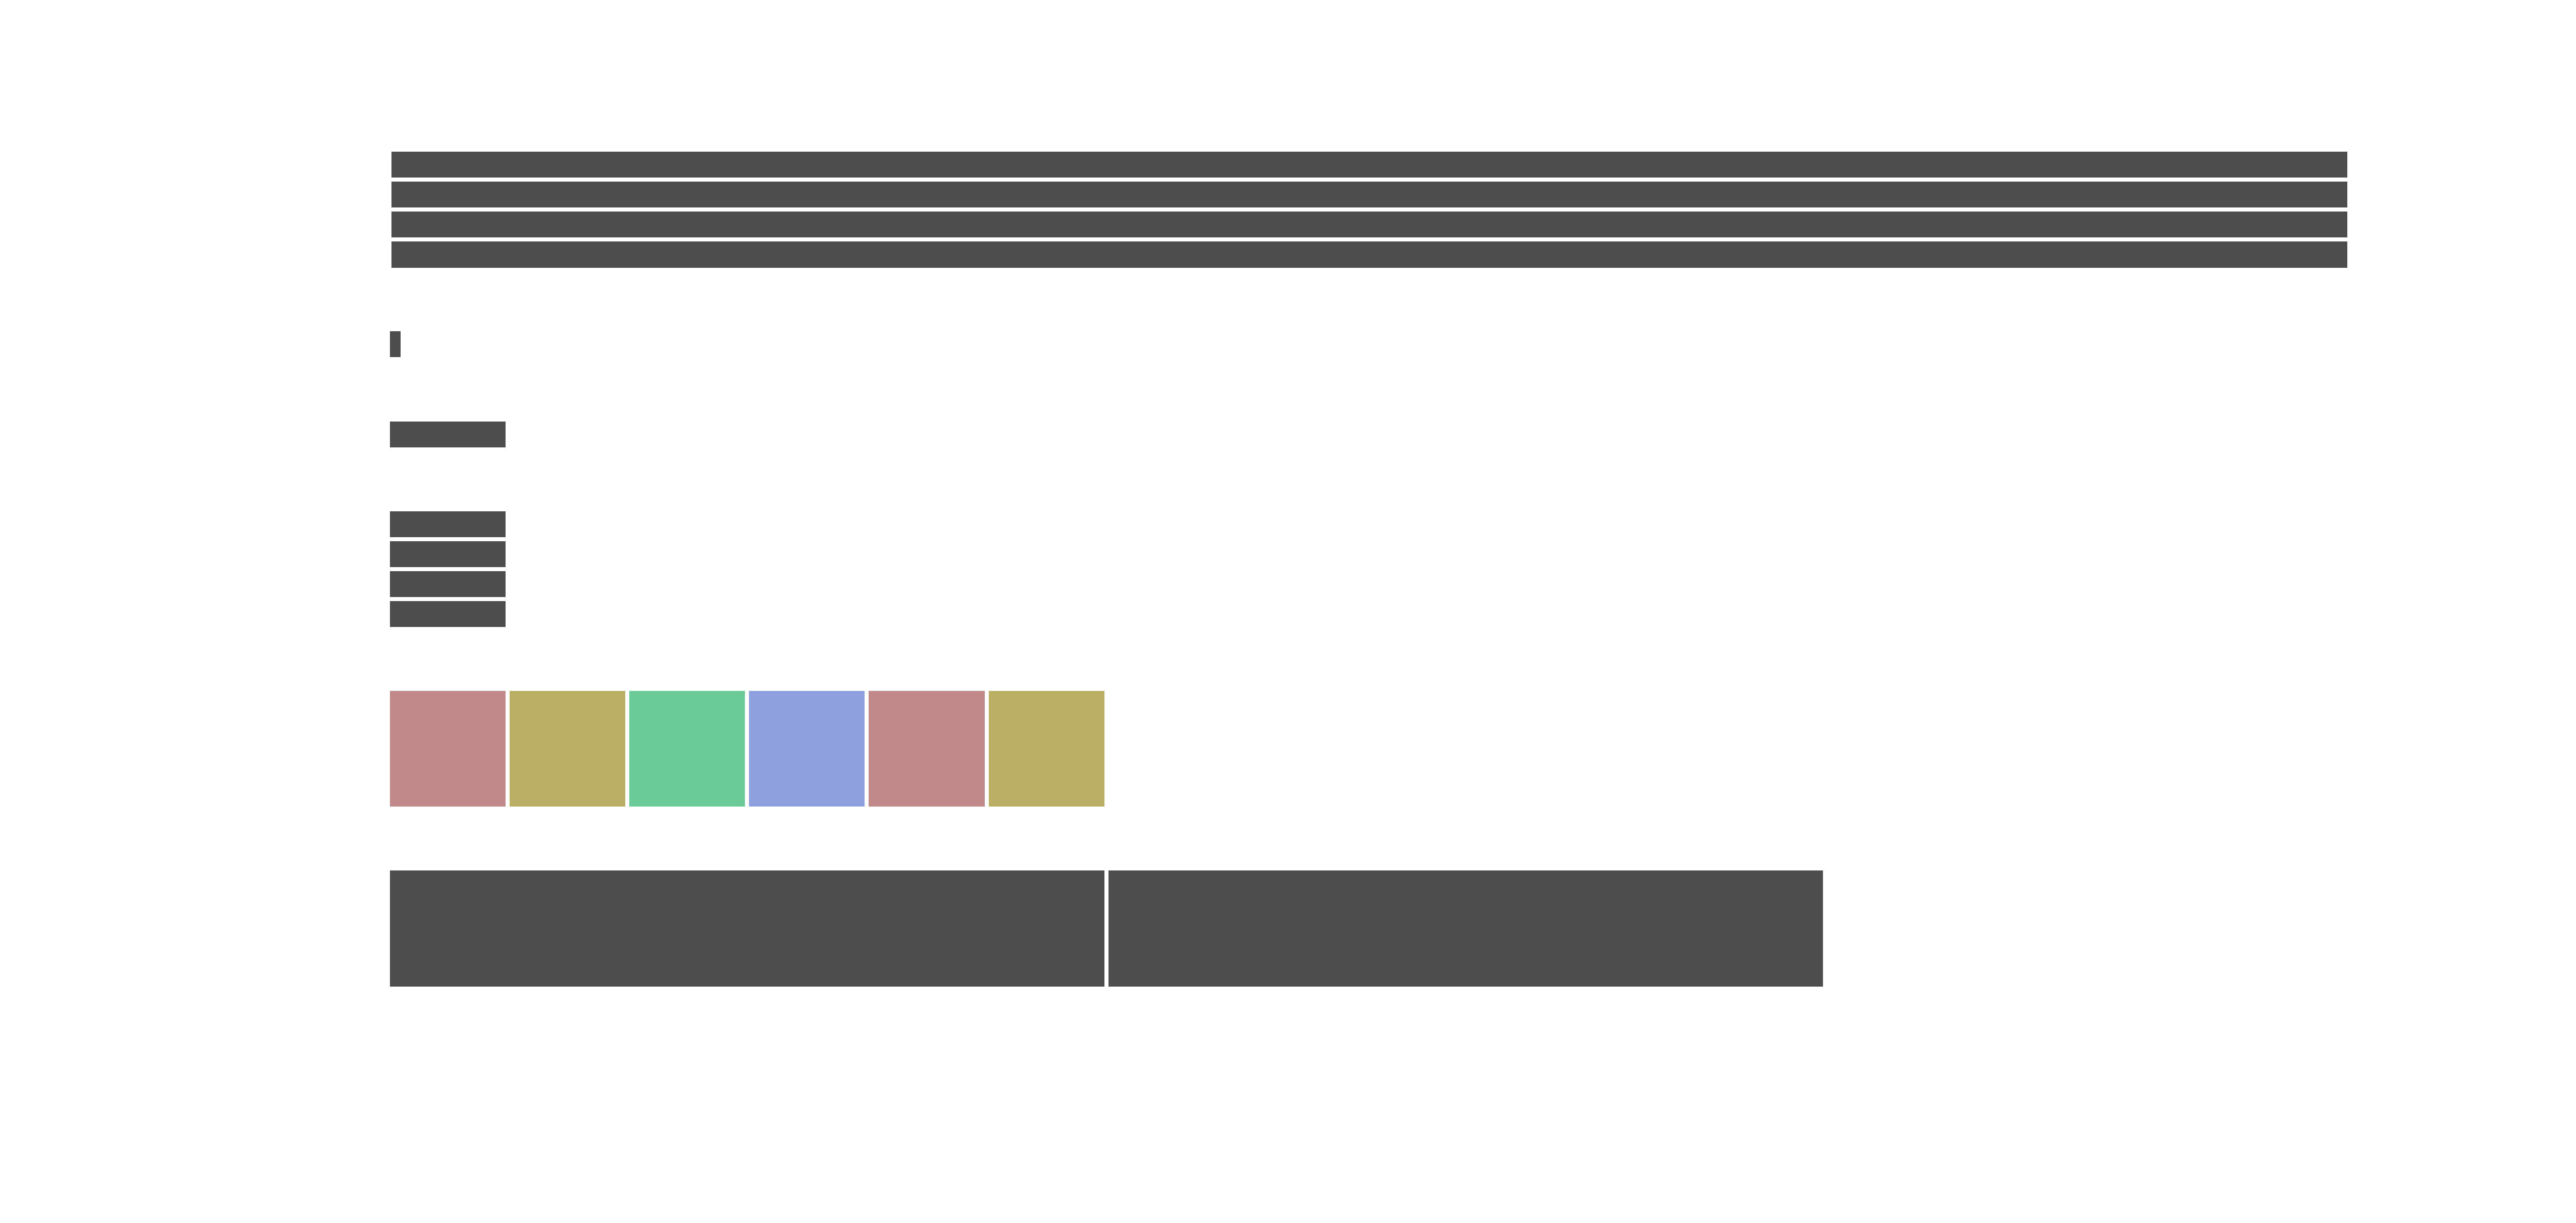
\includegraphics[width=1.0\textwidth]{cadence-4gpu}


\end{column}
\end{columns}

\end{frame}
\note{
}

%%%%%%%%%%%%%%%%%%%%%%%%%%%%%%%%%%%%%%%%%

\begin{frame}
\frametitle{GPT2 nano}

\begin{columns}[T]
\begin{column}[T]{0.6\textwidth}
\setlength{\parskip}{0.5em}

\vspace{1.0cm}
\begin{enumerate}
\setlength{\parskip}{0.5em}
\item Time to look at the code
\item Open your JupyterLab page
\item Connect to Jupyter
\item Open the {\tt train\_gpt2.py} file
\end{enumerate}

\end{column}
\begin{column}[T]{0.3\textwidth}
\setlength{\parskip}{0.5em}

\vspace{0.0cm}
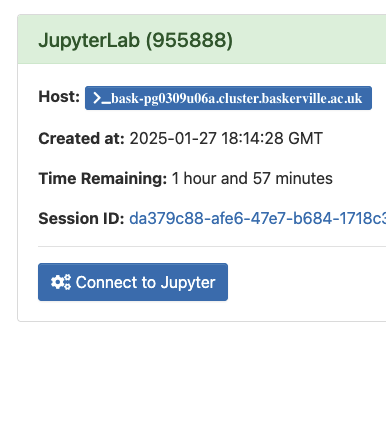
\includegraphics[width=1.0\textwidth]{connect-to-jupyter}

\end{column}
\end{columns}

\end{frame}
\note{
}

%%%%%%%%%%%%%%%%%%%%%%%%%%%%%%%%%%%%%%%%%

\begin{frame}
\frametitle{}

\begin{columns}[T]
\begin{column}[T]{1.0\textwidth}
\setlength{\parskip}{0.5em}

\vspace{0.0cm}
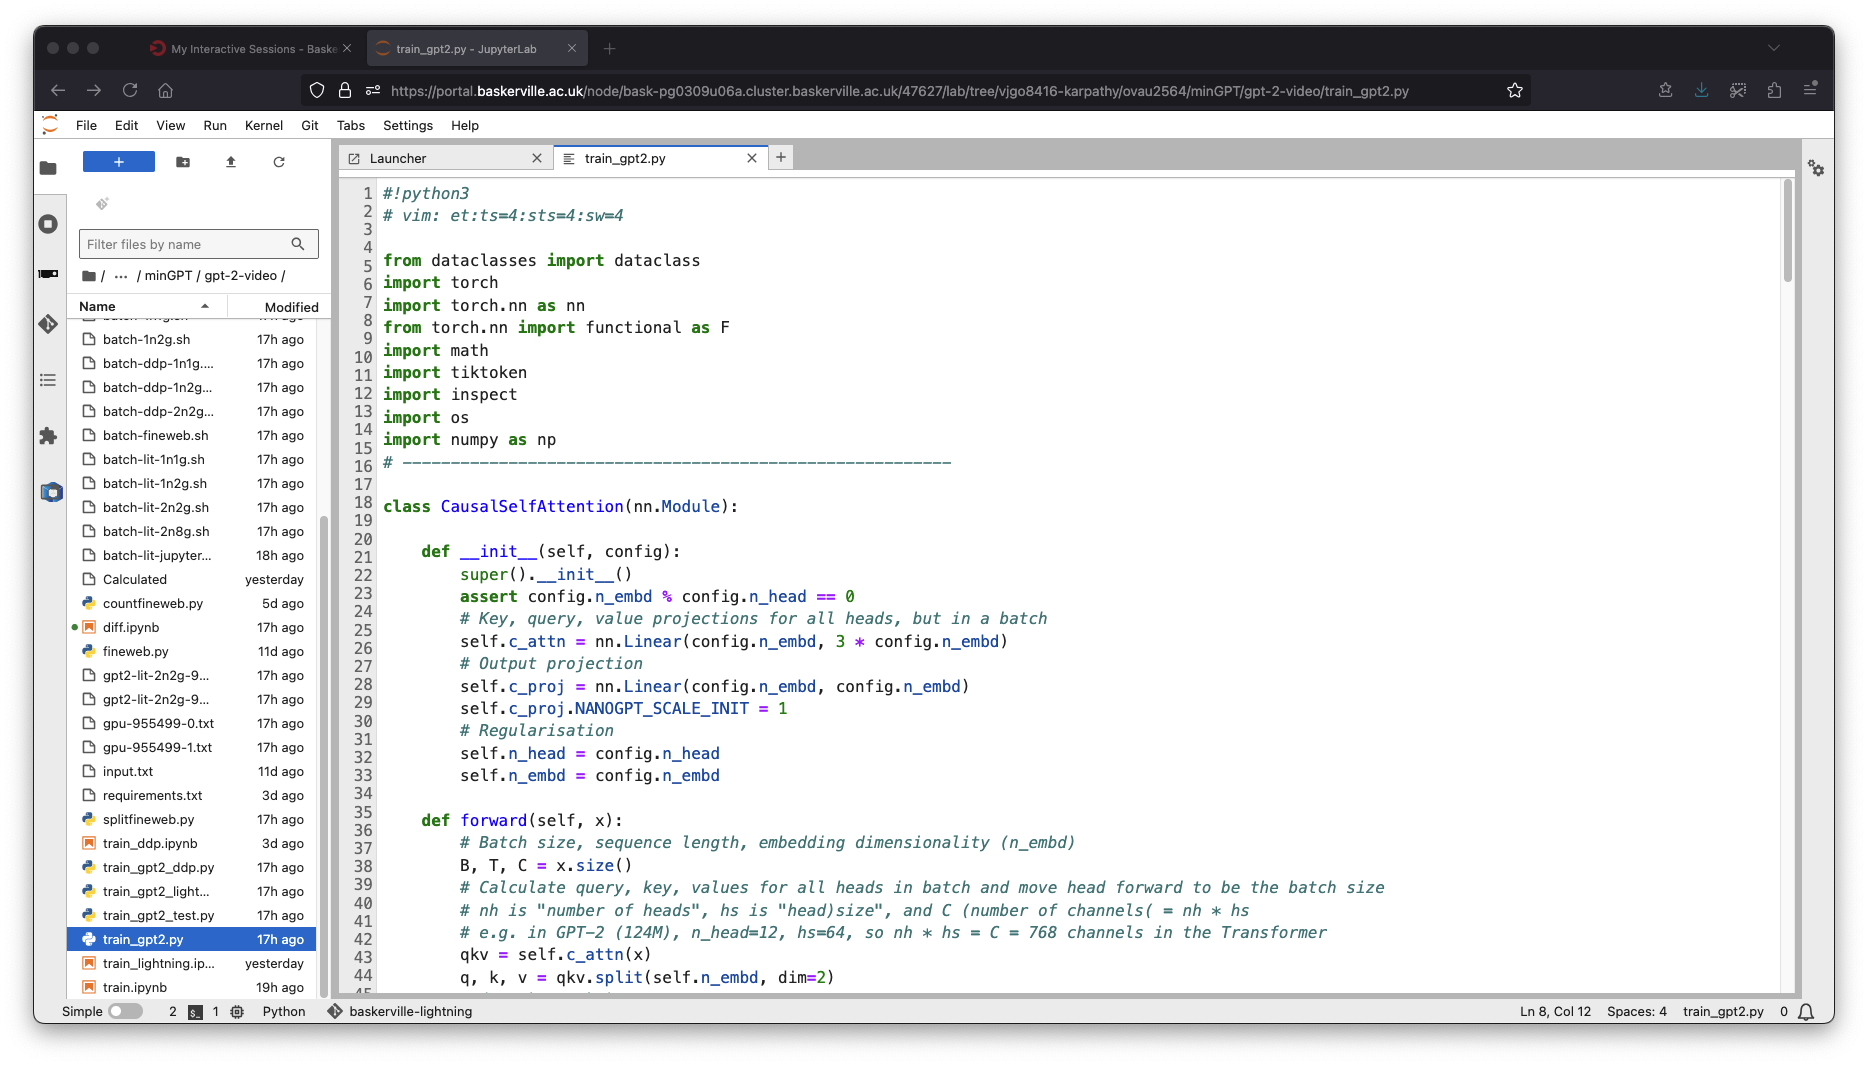
\includegraphics[width=1.0\textwidth]{traingpt2py}


\end{column}
\end{columns}

\end{frame}
\note{
}

%%%%%%%%%%%%%%%%%%%%%%%%%%%%%%%%%%%%%%%%%

\begin{frame}
\frametitle{GPT2 nano classes and functions}

\begin{columns}[T]
\begin{column}[T]{1.0\textwidth}
\setlength{\parskip}{0.5em}

\vspace{0.0cm}
\begin{enumerate}
\setlength{\parskip}{0.0em}
\item {\tt CausalSelfAttention}, {\tt MLP}, {\tt Block}: model components
\item {\tt GPTConfig}: model configuration
\item {\tt GPT}: the model
\item {\tt generate()}: inference
\item {\tt configure\_optimizers()}: training configuration
\item {\tt training\_step()}: one training step
\item {\tt load\_tokens()}: load a single FineWeb shard
\item {\tt get\_shards()}: find the FineWeb shards on disk
\item {\tt DataIterator}: our dataset and data loader
\item {\tt get\_lr()}: calculate the learning rate
\end{enumerate}

\end{column}
\end{columns}

\end{frame}
\note{
}

%%%%%%%%%%%%%%%%%%%%%%%%%%%%%%%%%%%%%%%%%

\begin{frame}
\frametitle{GPT2 nano execution}

\begin{columns}[T]
\begin{column}[T]{1.0\textwidth}
\setlength{\parskip}{0.5em}

\vspace{0.0cm}
\begin{enumerate}
\setlength{\parskip}{0.5em}
\item Set hyperparameters
\item Create model
\item Perform training loop
\end{enumerate}

\end{column}
\end{columns}

\end{frame}
\note{
}

%%%%%%%%%%%%%%%%%%%%%%%%%%%%%%%%%%%%%%%%%

\begin{frame}
\frametitle{Training time!}

\begin{columns}[T]
\begin{column}[T]{1.0\textwidth}
\setlength{\parskip}{0.5em}

\vspace{0.0cm}
\begin{enumerate}
\setlength{\parskip}{0.5em}
\item Right click on the {\tt train\_gpt2.py} tab
\item Select {\bf New View for Python File}
\item Open a {\bf GPU Resources} pane from the GPU Dashboard
\item Drag the pane to the tab space on the right
\item Open a terminal in the left tab space
\item {\tt source activate.sh}
\item {\tt python train\_gpt2.py}
\end{enumerate}

\end{column}
\end{columns}

\end{frame}
\note{
}

%%%%%%%%%%%%%%%%%%%%%%%%%%%%%%%%%%%%%%%%%

\begin{frame}
\frametitle{}

\begin{columns}[T]
\begin{column}[T]{1.0\textwidth}
\setlength{\parskip}{0.5em}

\vspace{0.0cm}
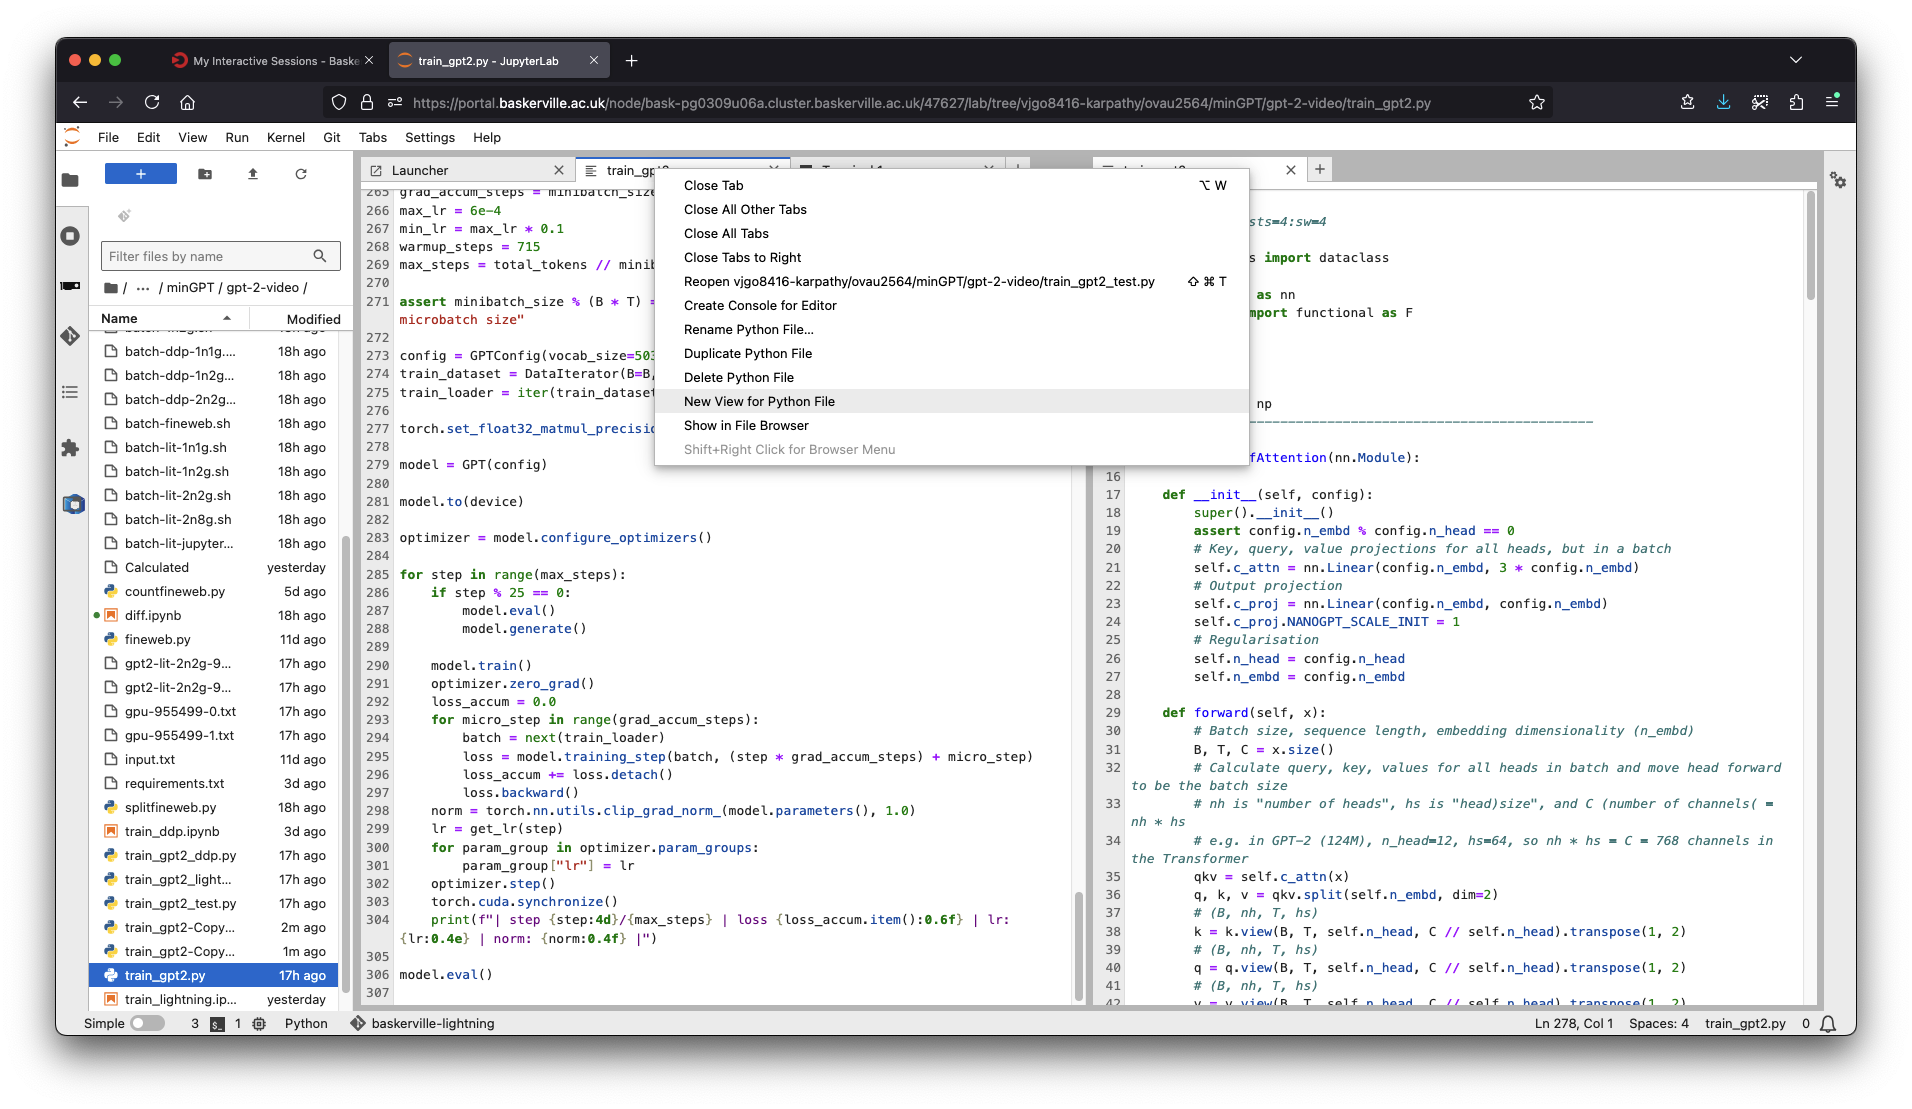
\includegraphics[width=1.0\textwidth]{execute01}


\end{column}
\end{columns}

\end{frame}
\note{
}

%%%%%%%%%%%%%%%%%%%%%%%%%%%%%%%%%%%%%%%%%

\begin{frame}
\frametitle{}

\begin{columns}[T]
\begin{column}[T]{1.0\textwidth}
\setlength{\parskip}{0.5em}

\vspace{0.0cm}
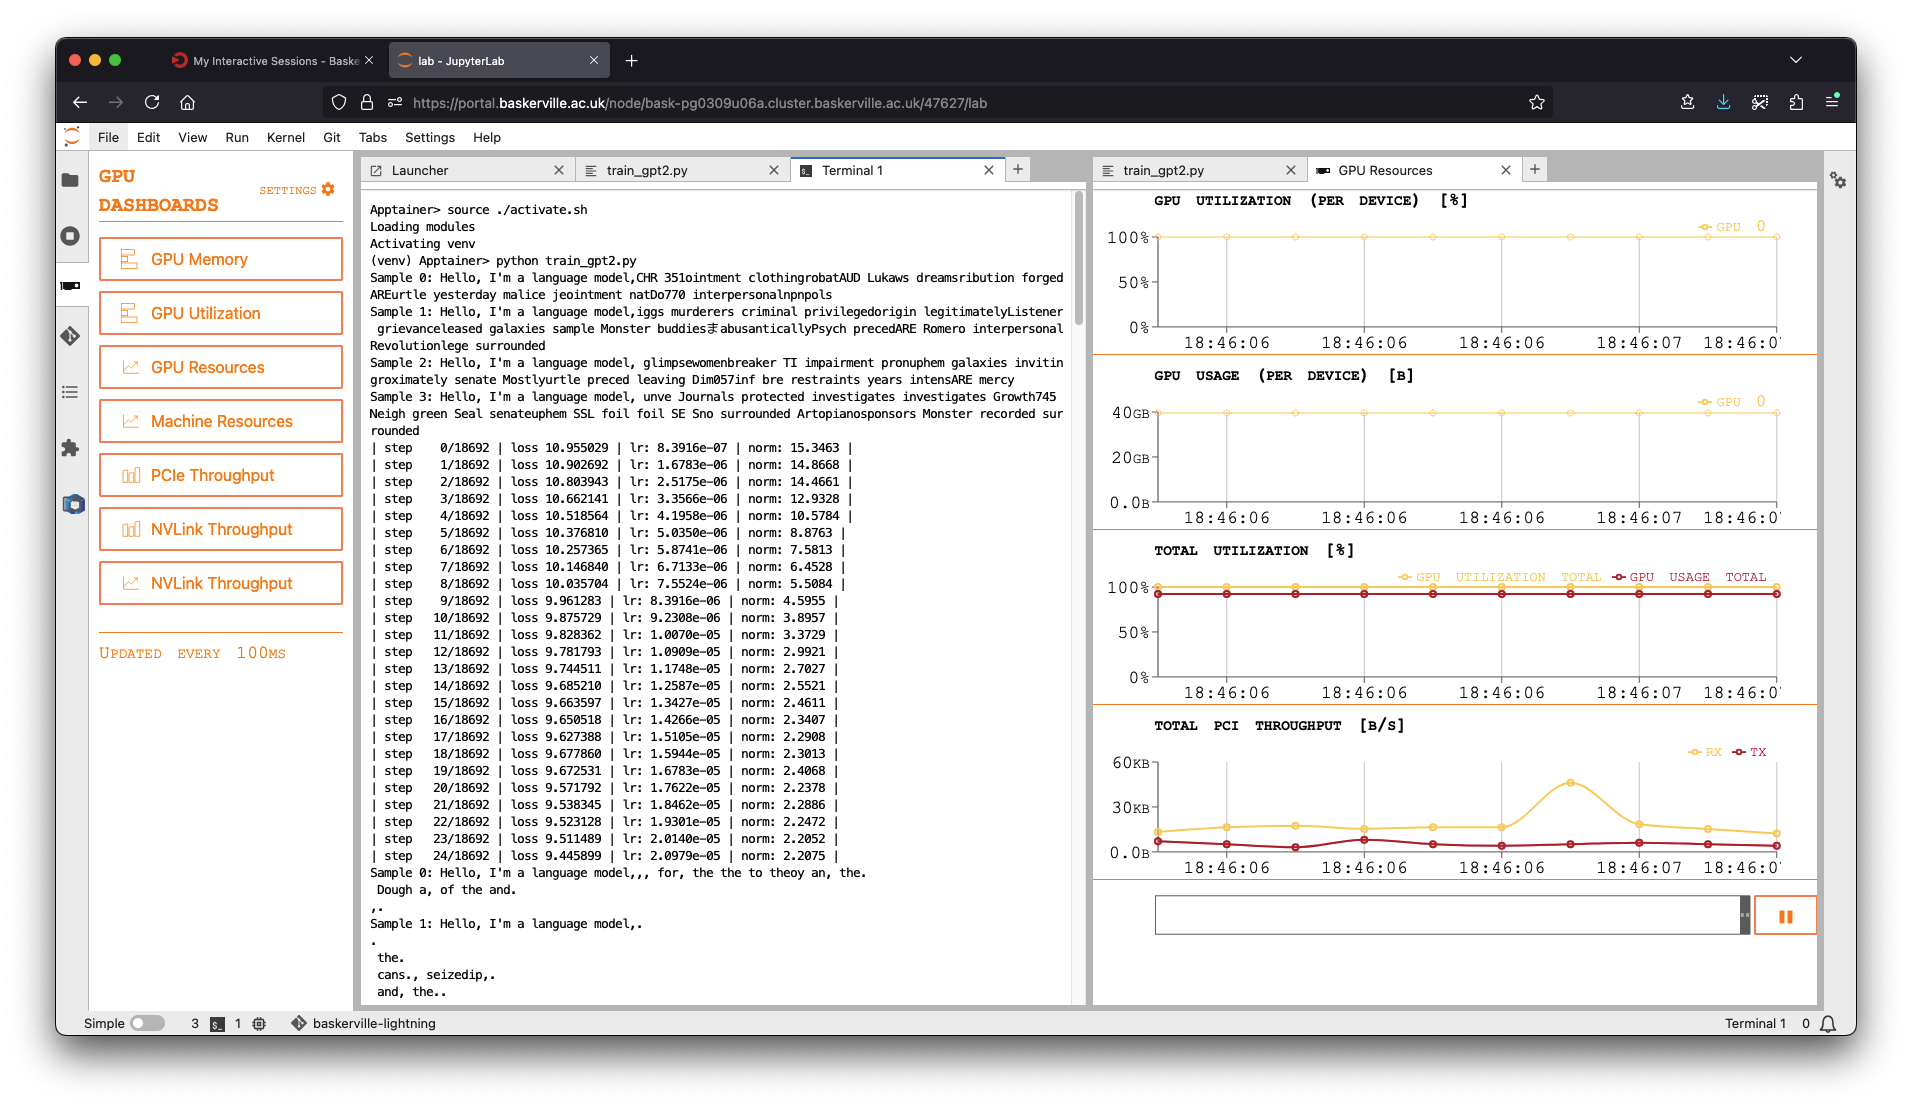
\includegraphics[width=1.0\textwidth]{execute02}


\end{column}
\end{columns}

\end{frame}
\note{
}

%%%%%%%%%%%%%%%%%%%%%%%%%%%%%%%%%%%%%%%%%

\begin{frame}
\frametitle{Upgrade to DDP}

\begin{columns}[T]
\begin{column}[T]{1.0\textwidth}
\setlength{\parskip}{0.5em}

\vspace{0.0cm}
\begin{enumerate}
\setlength{\parskip}{0.5em}
\item Open {\tt train\_gpt2.py} in the left hand tab space
\item Open {\tt diff\_ddp.ipynb} in the right hand tab space
\item Execute the first cell of {\tt diff\_ddp.ipynb}
\end{enumerate}

\end{column}
\end{columns}

\end{frame}
\note{
}

%%%%%%%%%%%%%%%%%%%%%%%%%%%%%%%%%%%%%%%%%

\begin{frame}
\frametitle{}

\begin{columns}[T]
\begin{column}[T]{1.0\textwidth}
\setlength{\parskip}{0.5em}

\vspace{0.0cm}
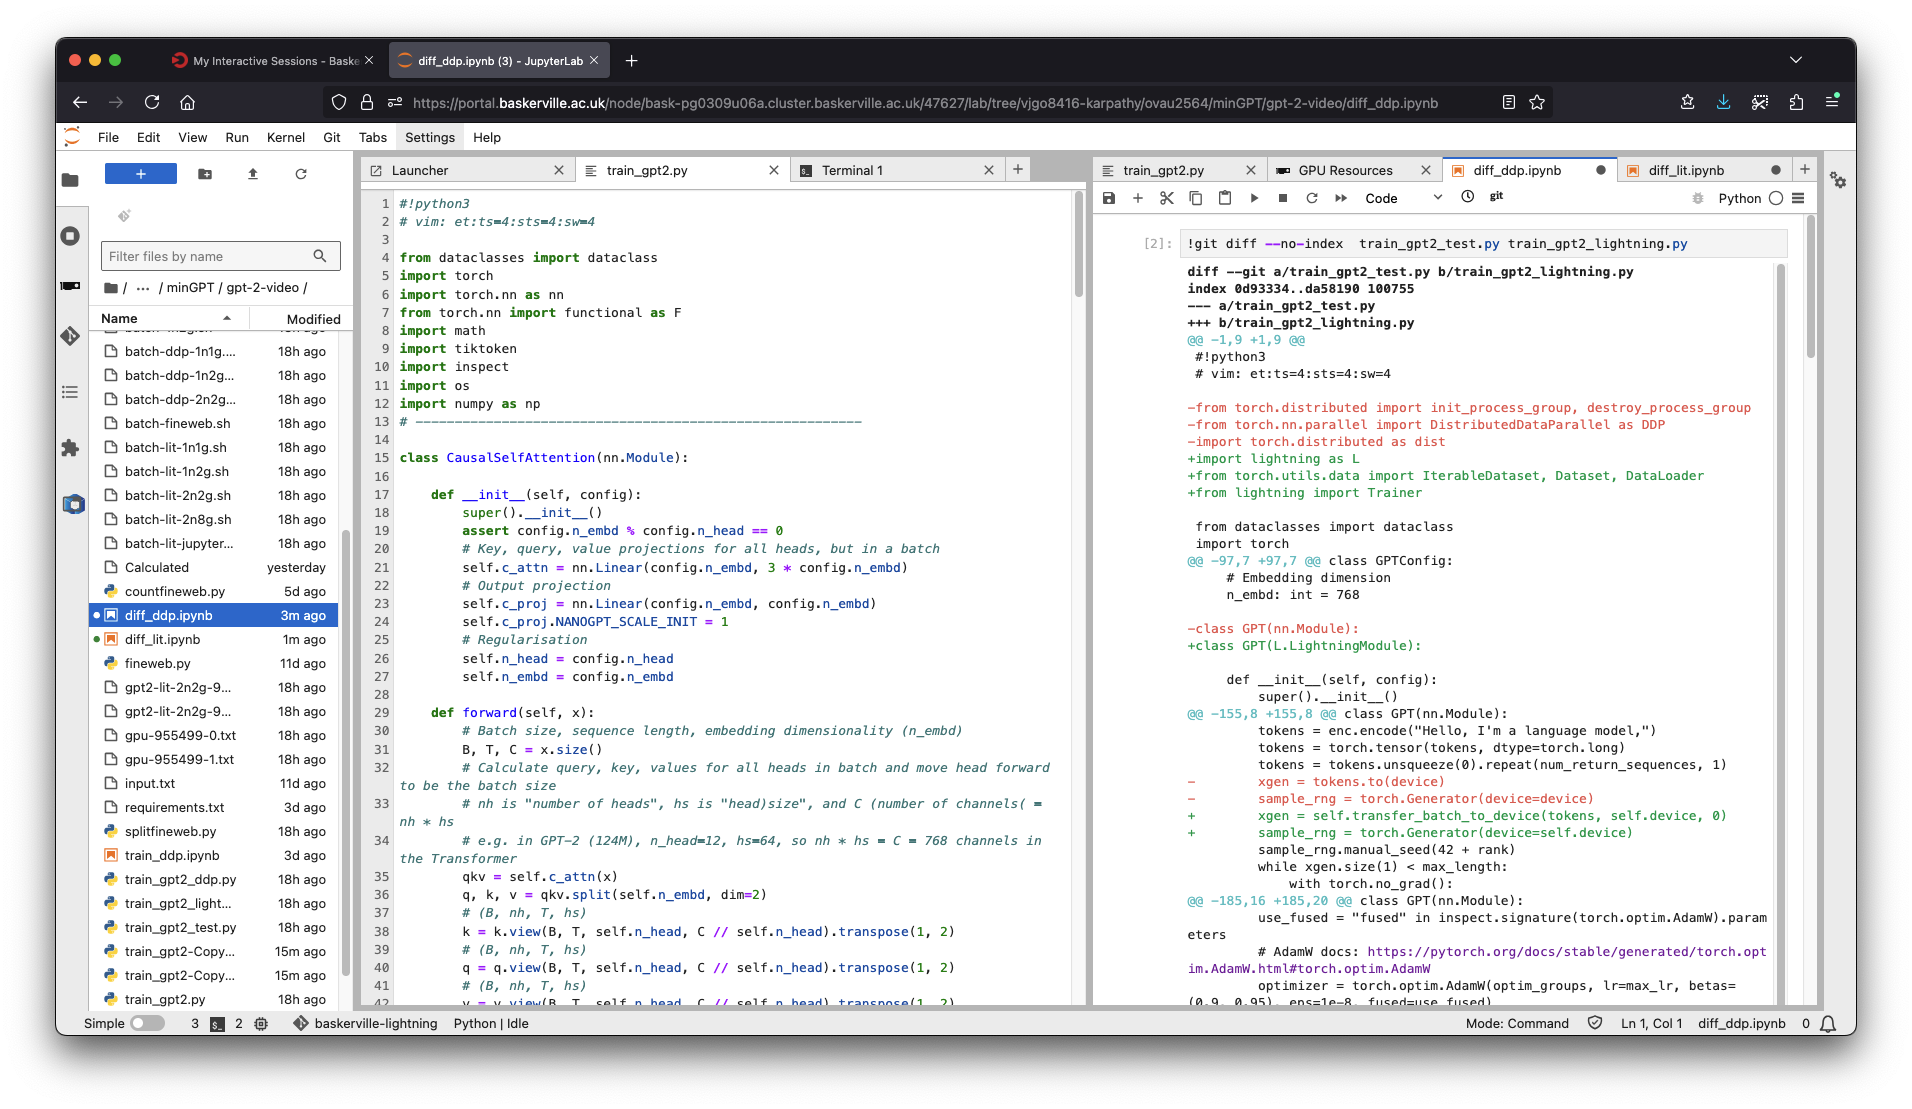
\includegraphics[width=1.0\textwidth]{diff01}


\end{column}
\end{columns}

\end{frame}
\note{
}

%%%%%%%%%%%%%%%%%%%%%%%%%%%%%%%%%%%%%%%%%

\begin{frame}
\frametitle{Understanding unified diffs}

\begin{columns}[T]
\begin{column}[T]{0.6\textwidth}
\setlength{\parskip}{0.5em}

\vspace{0.5cm}
\begin{enumerate}
\setlength{\parskip}{0.5em}
\item \textcolor{teal}{\tt @@} prefix indicates line numbers \\\textcolor{teal}{\tt @@ -before,len +after,len @@}
\item \textcolor{green}{\tt +} prefix in \textcolor{green}{green} indicates lines added
\item \textcolor{red}{\tt -} prefix in \textcolor{red}{red} indicates lines removed
\item Replay the cell to update the diff after making changes
\end{enumerate}

\end{column}
\begin{column}[T]{0.3\textwidth}
\setlength{\parskip}{0.5em}

\vspace{0.0cm}
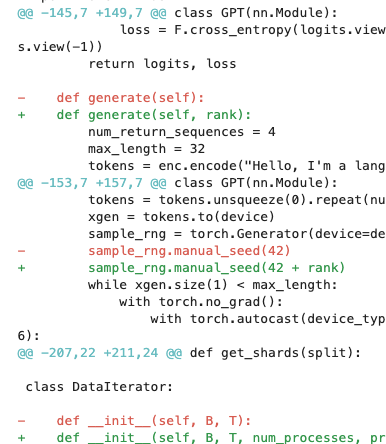
\includegraphics[width=1.0\textwidth]{diff02}

\end{column}
\end{columns}

\end{frame}
\note{
}

%%%%%%%%%%%%%%%%%%%%%%%%%%%%%%%%%%%%%%%%%

\begin{frame}
\frametitle{Manually apply the diff -- part I}

\begin{columns}[T]
\begin{column}[T]{1.0\textwidth}
\setlength{\parskip}{0.5em}

\vspace{0.0cm}
\begin{enumerate}
\setlength{\parskip}{0.0em}
\item Imports
\item One process per GPU
\item We {\it generate\/} on every process
\item One {\tt DataIterator} per GPU
\item We must shard the data appropriately
\item Initialise the process group
\item Harvest {\bf world size}, {\bf rank} and {\bf local rank} from the environment
\item Where do these come from?
\end{enumerate}

\end{column}
\end{columns}

\end{frame}
\note{
}

%%%%%%%%%%%%%%%%%%%%%%%%%%%%%%%%%%%%%%%%%

\begin{frame}
\frametitle{Manually apply the diff -- part II}

\begin{columns}[T]
\begin{column}[T]{1.0\textwidth}
\setlength{\parskip}{0.5em}

\vspace{0.0cm}
\begin{enumerate}
\setlength{\parskip}{0.0em}
\setcounter{enumi}{8}
\item Fix the gradient accumulation steps
\item Batch sizes must align
\item Create a {\tt DDP} model
\item Use the right model variable at the right time
\item Trigger backward gradient sync
\item Perform all reduce
\item Destroy the process group
\end{enumerate}

\end{column}
\end{columns}

\end{frame}
\note{
}

%%%%%%%%%%%%%%%%%%%%%%%%%%%%%%%%%%%%%%%%%

\begin{frame}
\frametitle{Observations}

\begin{columns}[T]
\begin{column}[T]{1.0\textwidth}
\setlength{\parskip}{0.5em}

\vspace{0.0cm}
\begin{enumerate}
\setlength{\parskip}{0.5em}
\item Most of this is boilerplate
\item The hardest part is sharding the data correctly
\item Because this is {\it data parallel}
\item MPI is also hard \\ \vspace{0.5em} \qquad \qquad \ldots but it's done for us by {\tt torch.distributed} and {\tt DDP}
\end{enumerate}

\end{column}
\end{columns}

\end{frame}
\note{
}

%%%%%%%%%%%%%%%%%%%%%%%%%%%%%%%%%%%%%%%%%

\begin{frame}[fragile]
\frametitle{Training time!}

\begin{columns}[T]
\begin{column}[T]{1.0\textwidth}
\setlength{\parskip}{0.5em}

\vspace{0.0cm}
\begin{enumerate}
\setlength{\parskip}{0.5em}
\item See {\tt batch-ddp-1n1g.sh} for single GPU
\item See {\tt batch-ddp-2n3g.sh} for dual-node dual GPU
\end{enumerate}

\begin{lstlisting}[backgroundcolor = \color{darkgray},language=shell]
# Single GPU
python -m torch.distributed.launch \
    --standalone --nproc_per_node=1 \
    train_gpt2_ddp.py

# Multi-node
python -m torch.distributed.launch \
    --nproc_per_node=${SLURM_GPUS_PER_NODE} \
    --nnodes=${SLURM_NNODES} \
    --master-port=${MASTER_PORT} --master-addr=${MASTER_ADDR} \
    train_gpt2_ddp.py
\end{lstlisting}

\end{column}
\end{columns}

\end{frame}
\note{
}

%%%%%%%%%%%%%%%%%%%%%%%%%%%%%%%%%%%%%%%%%

\begin{frame}
\frametitle{Upgrade to Lightning}

\begin{columns}[T]
\begin{column}[T]{1.0\textwidth}
\setlength{\parskip}{0.5em}

\vspace{0.0cm}
\begin{enumerate}
\setlength{\parskip}{0.5em}
\item Lightning is conceptually different
\item Code is organised in {\tt LightningModule}: init, train step, validation step, test step, optimisers
\item Code outside {\tt LightningModule} is automated by {\tt Trainer}
\item Remove code moving data to the GPU
\end{enumerate}

\end{column}
\end{columns}

\end{frame}
\note{
}
%%%%%%%%%%%%%%%%%%%%%%%%%%%%%%%%%%%%%%%%%

\begin{frame}
\frametitle{Upgrade to Lightning}

\begin{columns}[T]
\begin{column}[T]{1.0\textwidth}
\setlength{\parskip}{0.5em}

\vspace{0.0cm}
\begin{enumerate}
\setlength{\parskip}{0.5em}
\item Open {\tt train\_gpt2.py} in the left hand tab space
\item Open {\tt diff\_lit.ipynb} in the right hand tab space
\item Execute the first cell of {\tt diff\_lit.ipynb}
\end{enumerate}

\end{column}
\end{columns}

\end{frame}
\note{
}

%%%%%%%%%%%%%%%%%%%%%%%%%%%%%%%%%%%%%%%%%

\begin{frame}
\frametitle{Manually apply the diff -- part I}

\begin{columns}[T]
\begin{column}[T]{1.0\textwidth}
\setlength{\parskip}{0.5em}

\vspace{0.0cm}
\begin{enumerate}
\setlength{\parskip}{0.0em}
\item Imports
\item Switch from {\tt Module} to {\tt LightningModule}
\item Fix the {\tt generate()} function
\item Use the built-in {\tt OneCycleLR} learning rate scheduler
\item Remove CUDA code from {\tt training\_step()}
\item Generate examples periodically
\item Initialise {\tt DataIterator} using a {\tt worker\_init\_fn()}
\item Remove our custom learning rate scheduler code
\end{enumerate}

\end{column}
\end{columns}

\end{frame}
\note{
}

%%%%%%%%%%%%%%%%%%%%%%%%%%%%%%%%%%%%%%%%%

\begin{frame}
\frametitle{Manually apply the diff -- part II}

\begin{columns}[T]
\begin{column}[T]{1.0\textwidth}
\setlength{\parskip}{0.5em}

\vspace{0.0cm}
\begin{enumerate}
\setlength{\parskip}{0.0em}
\setcounter{enumi}{8}
\item Remove the process group code
\item Lose our DDP configuration
\item Simplify the random seeding
\item Fix the steps: minibatches are now implicit
\item Use a {\tt DataLoader} to sequence data loading
\item Remove our training loop
\item Add the {\tt Trainer} code
\end{enumerate}

\end{column}
\end{columns}

\end{frame}
\note{
}

%%%%%%%%%%%%%%%%%%%%%%%%%%%%%%%%%%%%%%%%%

\begin{frame}
\frametitle{Observations}

\begin{columns}[T]
\begin{column}[T]{1.0\textwidth}
\setlength{\parskip}{0.5em}

\vspace{0.0cm}
\begin{enumerate}
\setlength{\parskip}{0.5em}
\item The training code is greatly simplified
\item Lightning is SLURM-aware
\item So MPI is even easier
\item We can now switch to other strategies ({\it in theory})
\end{enumerate}

\end{column}
\end{columns}

\end{frame}
\note{
}

%%%%%%%%%%%%%%%%%%%%%%%%%%%%%%%%%%%%%%%%%

\begin{frame}[fragile]
\frametitle{Training time!}

\begin{columns}[T]
\begin{column}[T]{1.0\textwidth}
\setlength{\parskip}{0.5em}

\vspace{0.0cm}
\begin{enumerate}
\setlength{\parskip}{0.5em}
\item See {\tt batch-lit-2n8g.sh} for dual-node eight GPU
\item See {\tt batch-lit-jupyter.sh} to queue from Jupyter
\end{enumerate}

\begin{lstlisting}[backgroundcolor = \color{darkgray},language=shell]
# From inside a SLURM batch script
srun python train_gpt2_lightning.py

# Queue execution from inside JupyterLab
sbatch batch-lit-jupyter.sh
\end{lstlisting}

\end{column}
\end{columns}

\end{frame}
\note{
}

%%%%%%%%%%%%%%%%%%%%%%%%%%%%%%%%%%%%%%%%%

\begin{frame}
\frametitle{Scaling across nodes on A100 (40 GiB) GPUs}

\begin{columns}[T]
\begin{column}[T]{1.0\textwidth}
\setlength{\parskip}{0.5em}

\vspace{-1.5cm}
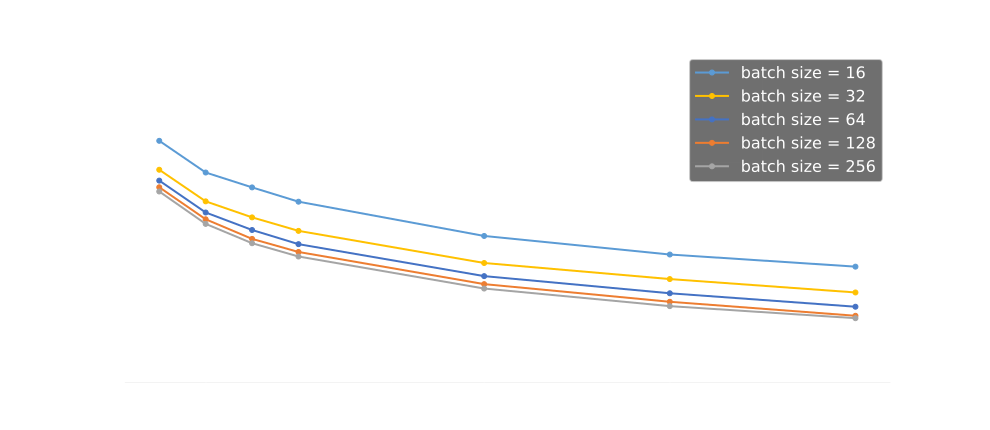
\includegraphics[width=1.0\textwidth]{scaling-a100}


\end{column}
\end{columns}

\end{frame}
\note{
}

%%%%%%%%%%%%%%%%%%%%%%%%%%%%%%%%%%%%%%%%%

\begin{frame}
\frametitle{Scaling across nodes on MX1550 (128 GiB) GPUs}

\begin{columns}[T]
\begin{column}[T]{1.0\textwidth}
\setlength{\parskip}{0.5em}

\vspace{-1.5cm}
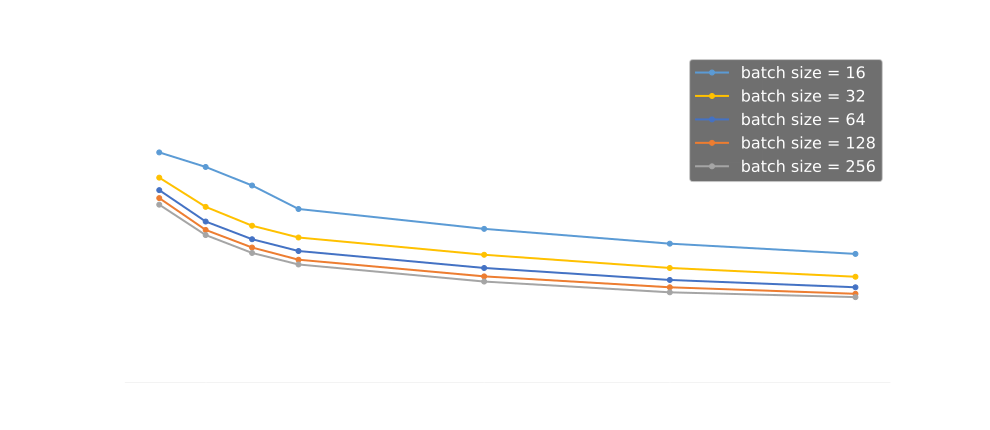
\includegraphics[width=1.0\textwidth]{scaling-mx1550}


\end{column}
\end{columns}

\end{frame}
\note{
}

%%%%%%%%%%%%%%%%%%%%%%%%%%%%%%%%%%%%%%%%%

\begin{frame}
\frametitle{Wrapping up}

\begin{columns}[T]
\begin{column}[T]{1.0\textwidth}
\setlength{\parskip}{0.5em}

\vspace{0.0cm}
\begin{enumerate}
\setlength{\parskip}{0.5em}
\item Converting code for distributed training is doable
\item Review and try out the batch scripts
\item More examples in the {\tt hpc-landscaptes} repository
\end{enumerate}

\vspace{0.5cm}
\qquad \url{https://github.com/alan-turing-institute/hpc-landscape}

\end{column}
\end{columns}

\end{frame}
\note{
}


%%%%%%%%%%%%%%%%%%%%%%%%%%%%%%%%%%%%%%%%%%

\end{document}
